%%%%%%%%%%%%%%%%%%%%%%%%%%%%%%%%%%%%%%%%%%%%%%%%%%%%%%%%%%%%%%%%%%%%%%%%%%%
%
% Plantilla para un artículo en LaTeX en español.
%
%%%%%%%%%%%%%%%%%%%%%%%%%%%%%%%%%%%%%%%%%%%%%%%%%%%%%%%%%%%%%%%%%%%%%%%%%%%

% Qué tipo de documento estamos por comenzar:
\documentclass[a4paper]{article}
% Esto es para que el LaTeX sepa que el texto está en español:
\usepackage[spanish]{babel}
\selectlanguage{spanish}
% Esto es para poder escribir acentos directamente:
\usepackage[utf8]{inputenc}
\usepackage[T1]{fontenc}



%% Asigna un tamaño a la hoja y los márgenes
\usepackage[a4paper,top=3cm,bottom=2cm,left=3cm,right=3cm,marginparwidth=1.75cm]{geometry}

%% Paquetes de la AMS
\usepackage{amsmath, amsthm, amsfonts}
%% Para añadir archivos con extensión pdf, jpg, png or tif
\usepackage{graphicx}
\usepackage[colorinlistoftodos]{todonotes}
\usepackage[colorlinks=true, allcolors=blue]{hyperref}

%% Primero escribimos el título
\title{Un algoritmo de dos fases para reconocer las actividades humanas en el contexto de la Industria 4. 0 y los procesos impulsados por el hombre}
\author{Borja Bordel$^1$, Ramón Alcarria$^1$, Diego Sánchez-de-Rivera$^1$\\
  \small $^1$Universidad Politécnica de Madrid, Madrid, España\\
  \small bbordel@dit.upm.es, ramon.alcarria@upm.es, diegosanchez@dit.upm.es\\
  \date{}
}

%% Después del "preámbulo", podemos empezar el documento

\begin{document}
%% Hay que decirle que incluya el título en el documento
\maketitle

%% Aquí podemos añadir un resumen del trabajo 
\begin{abstract}
\centering
Abstract.Los futuros sistemas industriales, una revolución conocida como Industria 4.0, están concebidos para integrar a las personas en el mundo cibernético como prosumidores (proveedores de servicios y consumidores). En este contexto, los procesos impulsados por el hombre aparecen como una realidad esencial y se necesitan instrumentos para crear circuitos de información de retroalimentación entre el subsistema social (personas) y el subsistema cibernético (componentes tecnológicos). Aunque se han propuesto muchos instrumentos diferentes, en la actualidad las técnicas de reconocimiento de patrones son las más prometedoras. Sin embargo, estas soluciones presentan algunos problemas importantes pendientes. Por ejemplo, dependen del hardware seleccionado para adquirir información de los usuarios; o presentan un límite en la precisión del proceso de reconocimiento. Para hacer frente a esta situación, en este trabajo se propone un algoritmo de dos fases para integrar a las personas en los sistemas de la Industria 4.0 y los procesos impulsados por el hombre. El algoritmo define acciones complejas como composiciones de movimientos simples. Las acciones complejas se reconocen utilizando modelos de Markov ocultos, y los movimientos simples se reconocen utilizando Dynamic Time Warping. De esta manera, sólo los movimientos dependen de los dispositivos de hardware empleados para capturar información, y la precisión del reconocimiento de acciones complejas se incrementa considerablemente. También se realiza una validación experimental real para evaluar y comparar el rendimiento de la solución propuesta.

Palabras Clave: Industria 4.0; reconocimiento de patrones; Warping Dinámico del Tiempo; Inteligencia Artificial; Modelos ocultos de Markov
\end{abstract}

%% Iniciamos "secciones" que servirán como subtítulos
%% Nota que hay otra manera de añadir acentos
\section{Introducci\'on}

Industria 4.0 [1] se refiere al uso de sistemas ciberfísicos (uniones de procesos físicos y cibernéticos) [2] como principal componente tecnológico de las futuras soluciones digitales, masculino (pero no sólo) en escenarios industriales. Típicamente, la digitalización ha provocado, al final, la sustitución de los mecanismos de trabajo tradicionales por nuevos instrumentos digitales. Por ejemplo, los trabajadores de las líneas de montaje fueron sustituidos por robots durante la tercera revolución industrial.
Sin embargo, algunas aplicaciones industriales no pueden basarse en soluciones tecnológicas, ya que el trabajo humano sigue siendo esencial [3]. Los productos hechos a mano son un ejemplo de aplicaciones en las que la presencia de obras humanas es esencial. En cualquier caso, estos sectores industriales deben integrarse también en la cuarta revolución industrial. De la unión de los Sistemas Cibernéticos Físicos (CPS) y los seres humanos actuando como proveedores de servicios (obras activas), surgen CPS humanizados [4]En estos nuevos sistemas se permiten procesos impulsados por el hombre [5], es decir, procesos que son conocidos, ejecutados y gestionados por personas (aunque pueden ser vigilados por mecanismos digitales).
Para crear una verdadera integración entre las personas y la tecnología, y trasladar la ejecución de los procesos del subsistema social (humanos) al mundo cibernético (componentes de hardware y software), se necesitan técnicas de extracción de información. En los últimos años se ha informado de muchas soluciones y enfoques diferentes, pero hoy en día las técnicas de reconocimiento de patrones son las más prometedoras.
El uso de Inteligencia Artificial, modelos estadísticos y otros instrumentos similares han permitido un desarrollo real e increíble de soluciones de reconocimiento de patrones, pero aún quedan algunos desafíos pendientes.
En primer lugar, las técnicas de reconocimiento de patrones dependen del dispositivo hardware subyacente para la captura de información. La estructura y el proceso de aprendizaje cambian si (por ejemplo) en lugar de los acelerómetros consideramos sensores infrarrojos. Esto es muy problemático ya que las tecnologías de hardware evolucionan mucho más rápido que las soluciones de software.
Y, segundo, hay un límite a la precisión en el proceso de reconocimiento. De hecho, a medida que las acciones humanas se vuelven más complicadas, se requieren más variables y modelos más complejos para reconocerlas. Este enfoque genera grandes problemas de optimización cuyo error residual es mayor a medida que aumenta el número de variables, lo que provoca una disminución de la tasa de reconocimiento de éxito [6]. En conclusión, las matemáticas (no el software, por lo tanto, no depende de la implementación) obligan a una cierta precisión en el proceso de reconocimiento de patrones dadas las acciones a estudiar. Para evitar esta situación, se debe considerar un menor número de variables, pero también se reduce la complejidad de las acciones que se pueden analizar, lo que resulta inaceptable en escenarios industriales donde se desarrollan actividades productivas complejas.
Por lo tanto, el objetivo de este trabajo es describir un nuevo algoritmo de reconocimiento de patrones que aborde estos dos problemas básicos. El mecanismo propuesto define las acciones como una composición de simples movimientos. Los movimientos simples se reconocen mediante técnicas de Warping Dinámico del Tiempo (DTW) [7]. Este proceso depende del hardware seleccionado para la captura de información; pero las DTW son muy flexibles y actualizar el repositorio de patrones es suficiente para reconfigurar todo el algoritmo. Luego, las acciones complejas se reconocen como combinaciones de movimientos simples a través de los Modelos Ocultos de Markov (HMM) [8]. Estos modelos son totalmente independientes de las tecnologías de hardware, ya que solo consideran acciones simples. Este enfoque en dos fases también reduce la complejidad de los modelos, aumentando la precisión y la tasa de éxito en el proceso de reconocimiento.
El resto del trabajo está organizado de la siguiente manera: en la sección 2 se describe el estado de la técnica en el reconocimiento de patrones para actividades humanas; en la sección 3 se describe la solución propuesta, incluidas las dos fases definidas; en la sección 4 se presenta una validación experimental utilizando un escenario real y usuarios finales; y en la sección 5 se concluye el trabajo.

\section{Algunos ejempllos para comenzar}

\subsection{¿Cómo incluir figuras?}

Primero tienes que cargar el archivo de imagen desde su computadora usando el enlace de carga del menú del proyecto. Luego usando el comando 'includegraphics' podrás incluirlo en el documento. Con el entorno de figura y el comando de título podrás agregar un número y un título a la figura. Mira el código de la Figura \ref{fig:tesla} en esta sección para ver un ejemplo.

\begin{figure}
\centering
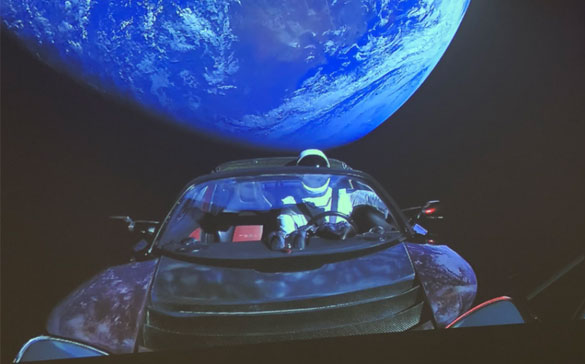
\includegraphics[width=0.5\textwidth]{tesla.jpg}
\caption{\label{fig:tesla}Esta imagen se añadió en el menú Project.}
\end{figure}


\subsection{¿Cómo añadir comentarios?}
% * <stephmigoni@gmail.com> 2018-02-08T19:23:33.559Z:
% 
% Esto es un comentario de prueba
% 
% 

Puedes añadir comentarios en el ícono + del menú de arriba.

Para responder a un comentario, simplemente da click en Reply en Rich Text.

También pueden añadirse comentarios en el margen del pdf compilado con el comando todo \todo{¡Comment en el margen!}, como se muestra en el ejemplo de la derecha. También puedes añadirlos dentro del texto:

\todo[inline, color=green!40]{Este es un comentario dentro del texto.}

\subsection{¿Cómo añadir tablas en mi \TeX?}

Usa los comandos table y tabular para iniciar una tabla simple --- mira la tabla~\ref{tab:tabla ejemplo}, como ejemplo. 

\begin{table}
\centering
\begin{tabular}{l c r} 
%nùmero de columnas: 3
l para left & c para centro & r para derecha \\ \hline
Ejemplo & Centrado & Alineado a la\\
Izquierda & 13 & Derecha
\end{tabular}
\caption{\label{tab:tabla ejemplo}Una simple tabla.}
\end{table}

\subsection{¿Cómo escribir (expresiones) Matemáticas?}

\LaTeX{} es buenísimo para escribir ecuaciones. Para escribir variables o ecuaciones dentro del texto lo podemos poner entre signos de pesos y luego podemos seguir escribiendo, esto funciona si queremos escribir un símbolo como $\nabla$, $\pi$, $\beta$, $\Omega$, $\aleph$, etc.
\begin{equation}
\sum_{n=0}^\infty \frac{x^n}{n!}=e^x
\end{equation}
\begin{equation}
\int_{0}^{1}dx=1
\end{equation}
\begin{equation}
e^{i\pi}+1=0
\end{equation}
Si queremos citar al gran Maxwell, lo podemos hacer como en la ecuación \ref{eq:Maxwell}:
\begin{equation}
\nabla\times\mathbf{E}+\frac{\partial\mathbf{B}}{\partial t}=0\label{eq:Maxwell}
\end{equation}

A continuación se añade un ejemplo de un desarrollo:
Con este preámbulo llevamos a cabo la siguiente transformación de los operadores $\hat{a}_{\ell}$

\begin{equation}
\hat{b}_{m}^{\dagger}=\sum_{\ell}U_{m}^{\ell}\hat{a}_{\ell}^{\dagger}
\end{equation}

donde $U_{m}^{\ell}$ es un elemento de la matriz unitaria $\mathbf{U}$.

Calculamos ahora su hermitiano conjugado
\begin{align}
\hat{b}_{m} & =\left(\sum_{\ell}U_{m}^{\ell}\hat{a}_{\ell}^{\dagger}\right)^{\dagger}\label{eq:bm}\\
 & =\sum_{\ell}\left(U_{m}^{\ell}\hat{a}_{\ell}^{\dagger}\right)^{\dagger}\nonumber \\
 & =\sum_{\ell}\left(U_{m}^{\ell}\right)^{*}\hat{a}_{\ell}\nonumber \\
 & =\sum_{\ell}\left(U^{-1}\right)_{\ell}^{m}\hat{a}_{\ell},\label{eq:bSubM}
\end{align}

Ahora, para añadir una matriz:

$$
\begin{matrix} 
a & b \\
c & d 
\end{matrix}
\quad
\begin{pmatrix} 
a & b \\
c & d 
\end{pmatrix}
\quad
\begin{bmatrix} 
a & b \\
c & d 
\end{bmatrix}
\quad
\begin{vmatrix} 
a & b \\
c & d 
\end{vmatrix}
\quad
\begin{Vmatrix} 
a & b \\
c & d 
\end{Vmatrix}
$$
%% Por ejemplo, el triple producto escalar:
\begin{equation}
\vec{A}\cdot(\vec{B}\times\vec{C})=\begin{vmatrix}
A_x&A_y&A_z\\
B_x&B_y&B_z\\
C_x&C_y&C_z\\
\end{vmatrix}
\end{equation}

\subsection{¿Cómo añadir listas?}

Puedes añadir listas con numeración automática \dots

\begin{enumerate}
\item Como esta,
\item y como esta.
\end{enumerate}
\dots o con puntitos \dots
\begin{itemize}
\item Como este,
\item y como este.
\end{itemize}

\subsection{¿Cómo añado una lista de Citas y Referencias?}

Puedes subir un archivo \verb|.bib| que contenga todas tus referencias en estilo BibTeX (puedes buscar la bibliografía de un libro en google añadiendo 'bibtex' al final), creado con JabRef. Luego podrás hacer citas así: \cite{Griffiths:1492149}.

Puedes encontrar un \href{https://www.overleaf.com/help/97-how-to-include-a-bibliography-using-bibtex}{video tutorial aquí} para aprender más acerca de BibTeX.

Espero que esta charla haya sido de tu ayuda. Puedes acceder a Overleaf en el siguiente link: \url{https://www.overleaf.com/}!

\bibliographystyle{abbrv}
\bibliography{sample}

\end{document}